\section{History of the project}\label{sec:history-of-the-project}
This project originally began in January 2023 as work for a paper~\cite{keyrtual} presented at the 20th International
Conference on Computer Analysis of Images and Patterns (CAIP 2023).
While the paper's version and the current version of the project are similar in purpose, they are completely different in implementation.
The main difference between the two is that the first one was not intended for mobile devices, but was essentially
a prototype designed to assess the general feasibility of the project,
although it was still meant to be suitable for low-end (non-mobile) devices.

In this first prototype, the procedure to use the program is longer and more cumbersome, and is summarized
in~\autoref{fig:keyrtual-leap-motion-method}.

\begin{figure}
	\center
	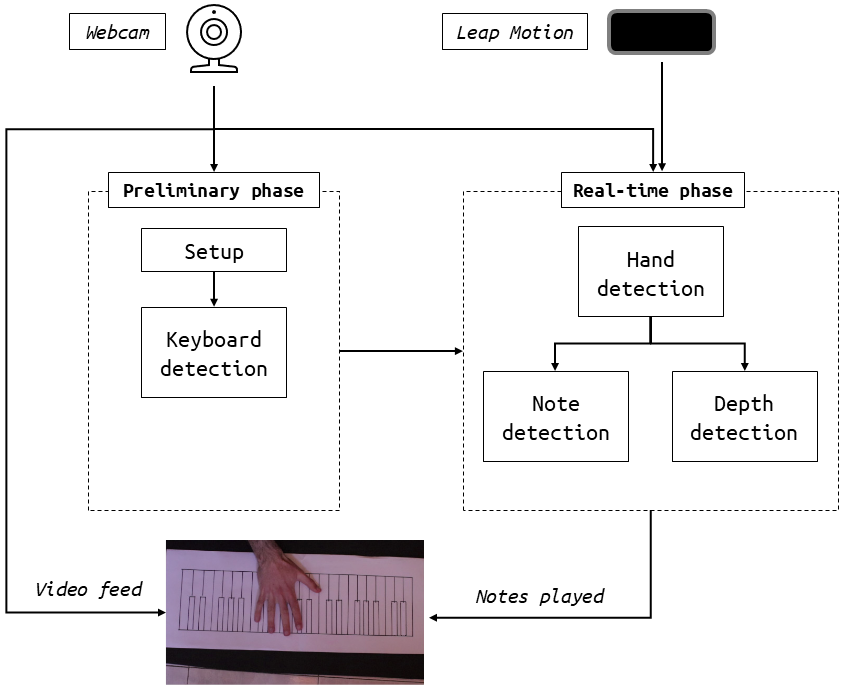
\includegraphics[width=0.8\textwidth]{first-prototype-architecture}
	\caption{Architecture of the first prototype}
	\label{fig:keyrtual-leap-motion-method}
\end{figure}

\subsection{Constraints}\label{subsec:constraints-prototype}

\paragraph{General constraints}
The paper sheet where the keyboard is drawn should have a sufficiently strong
contrast to the table, and the same applies to the keys drawn to the paper.

The camera and Leap Motion should also be placed at an adeguate distance
to be able to frame the paper and hands in their entirety.
They should be placed perpendicular to the table, so that they have as good a view as possible from above,
and oriented so that the user appears at the top.

\paragraph{Hardware prerequisites}
First, the use of an external webcam and a Leap Motion Controller is required.
These two devices should be placed next to each other perpendicular to the table on which the user intends to
use the drawn keyboard, so as to have an elevated view of the keyboard and the user's hands.

As for the computer, there is no special prerequisite since the program is designed to
be used even on low-end devices.

\subsection{Preliminary phase}\label{subsec:preliminary-phase-prototype}
The preliminary phase is divided into two parts: the background subtraction part and the keyboard detection part.
The whole process is illustrated in~\autoref{fig:preprocessing-prototype}

\paragraph{Background subtraction}
Once the components are assembled, we move on to the preliminary stage of keyboard detection.
For this purpose, a background subtraction operation is first performed, which consists of taking two pictures:
the first will be a picture of the table without the keyboard, while the second will include the keyboard.
By calculating the differences between the two images, the background is removed, leaving only the keyboard.

\paragraph{Keyboard detection}
Once the area of the image on which the keyboard is located has been identified, we proceed with key detection.
This is done by applying different filters to the image to increase the contrast between white sheet and black keys,
and using classic algorithms such as Canny edge detector, probabilistic Hough Transform procedure
and K-means clustering to extrapolate the rows that make up the keyboard keys.
These rows are separated according to their length and position to separately identify white keys and black keys.

\begin{figure}[t]
	\centering
	\begin{subfigure}{0.32\textwidth}
		\centering
		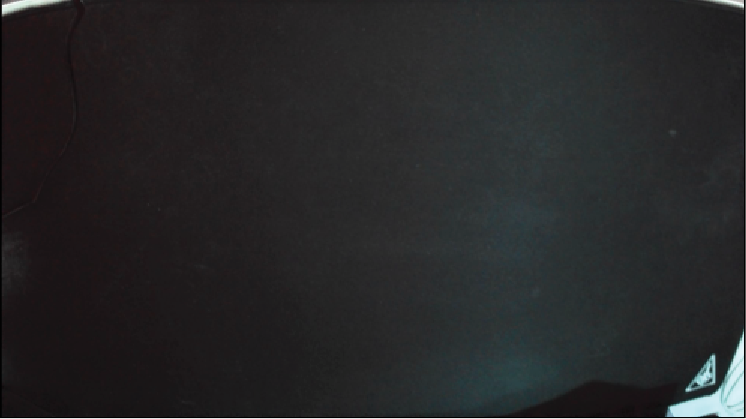
\includegraphics[width=\textwidth]{prototype-method/setup-1}
		\caption{}
		\label{fig:setup_background}
	\end{subfigure}
	\hfill
	\begin{subfigure}{0.32\textwidth}
		\centering
		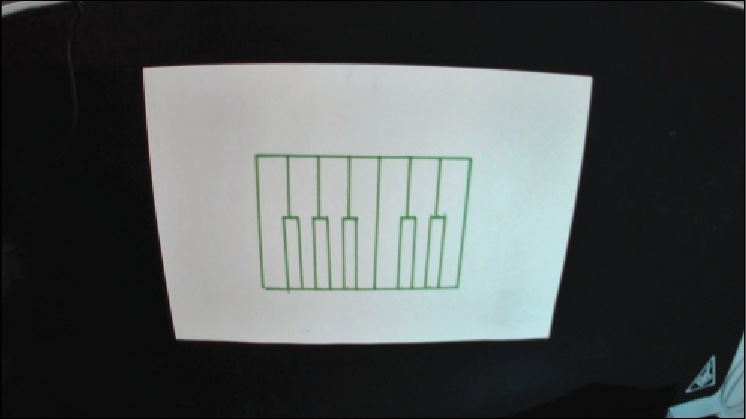
\includegraphics[width=\textwidth]{prototype-method/setup-2}
		\caption{}
		\label{fig:setup_keyboard}
	\end{subfigure}
	\hfill
	\begin{subfigure}{0.32\textwidth}
		\centering
		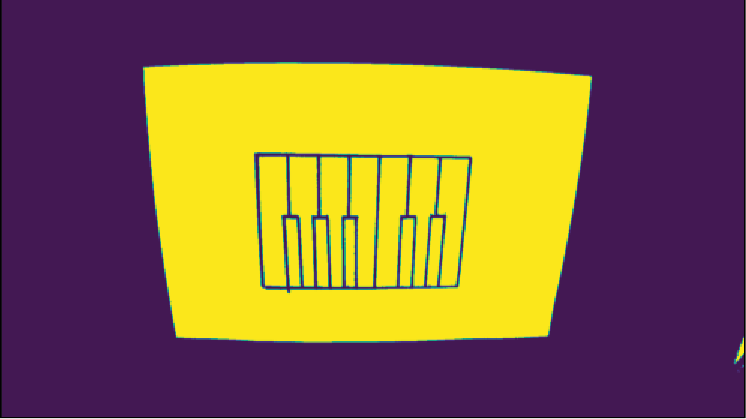
\includegraphics[width=\textwidth]{prototype-method/background}
		\caption{}
		\label{fig:keyboard_background}
	\end{subfigure}
	\hfill
	\begin{subfigure}{0.32\textwidth}
		\centering
		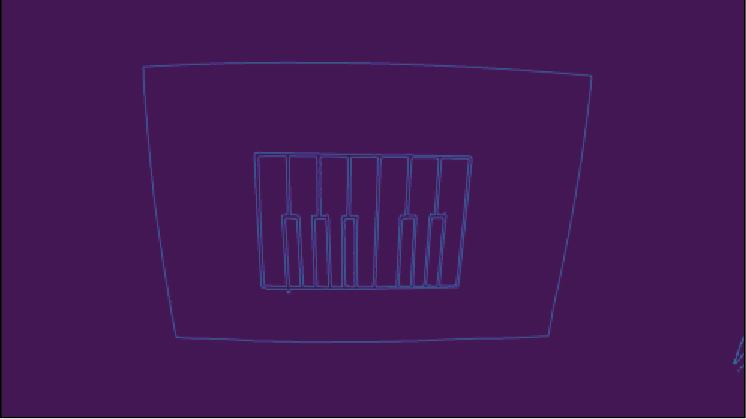
\includegraphics[width=\textwidth]{prototype-method/edges}
		\caption{}
		\label{fig:canny-prototype}
	\end{subfigure}
	\hfill
	\begin{subfigure}{0.32\textwidth}
		\centering
		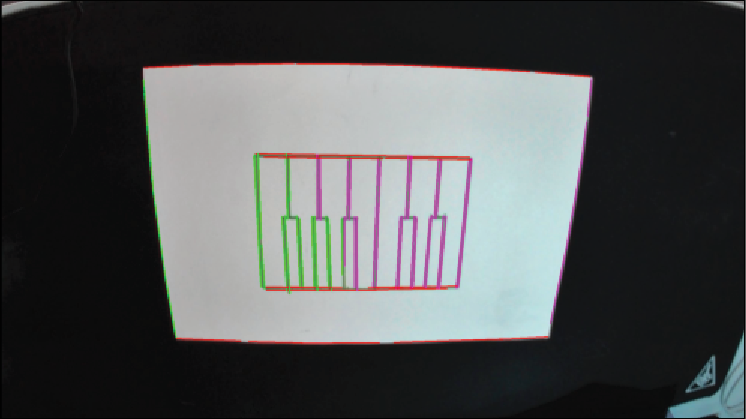
\includegraphics[width=\textwidth]{prototype-method/lines}
		\caption{}
		\label{fig:hough}
	\end{subfigure}
	\hfill
	\begin{subfigure}{0.32\textwidth}
		\centering
		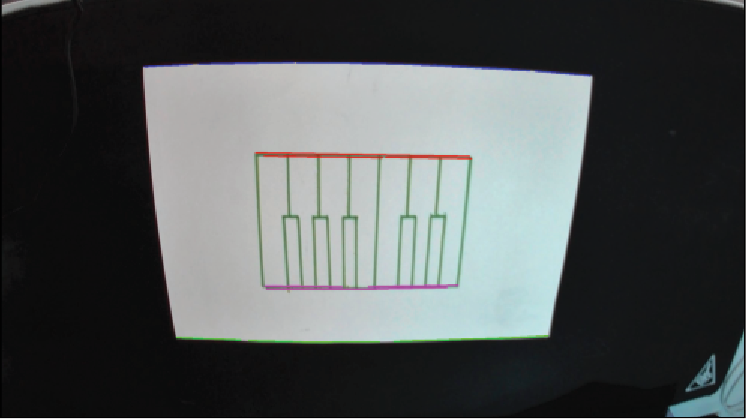
\includegraphics[width=\textwidth]{prototype-method/hor-lines}
		\caption{}
		\label{fig:hor_lines}
	\end{subfigure}
	\hfill
	\begin{subfigure}{0.32\textwidth}
		\centering
		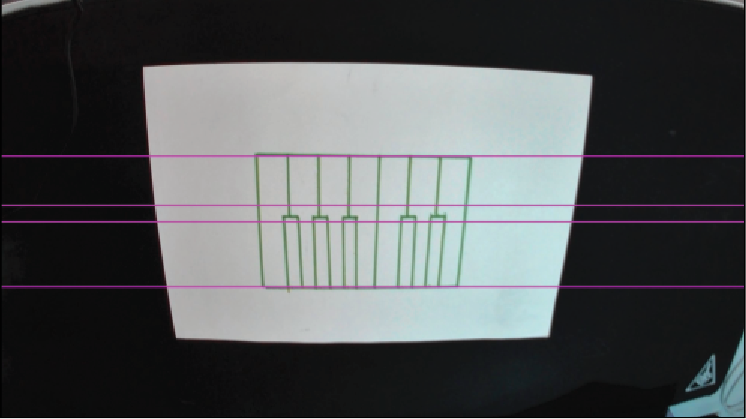
\includegraphics[width=\textwidth]{prototype-method/borders}
		\caption{}
		\label{fig:borders}
	\end{subfigure}
	\hfill
	\begin{subfigure}{0.32\textwidth}
		\centering
		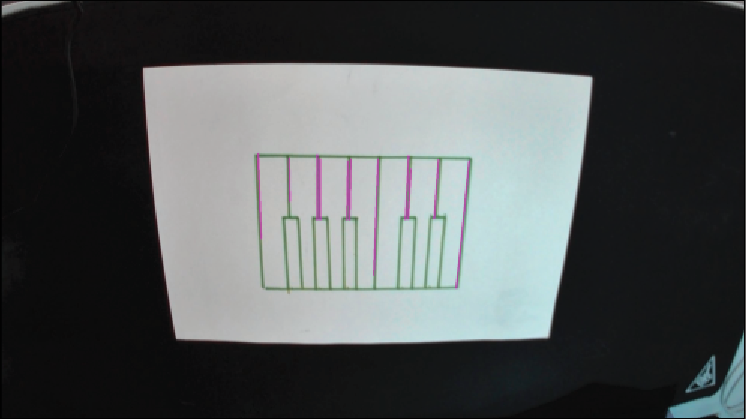
\includegraphics[width=\textwidth]{prototype-method/white-tiles}
		\caption{}
		\label{fig:white_tiles}
	\end{subfigure}
	\hfill
	\begin{subfigure}{0.32\textwidth}
		\centering
		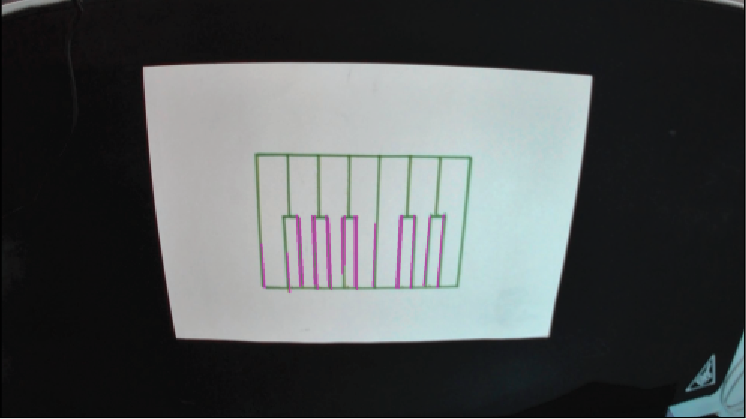
\includegraphics[width=\textwidth]{prototype-method/black-tiles}
		\caption{}
		\label{fig:black_tiles}
	\end{subfigure}
	\caption{
		Preliminary phase pipeline.
		(a) First frame;
		(b) Second frame;
		(c) Background highlight;
		(d) Canny edge detection;
		(e) Hough transformation;
		(f) Horizontal lines detection;
		(g) Borders highlight;
		(h) White tiles highlight;
		(i) Black tiles highlight.
	}
	\label{fig:preprocessing-prototype}
\end{figure}

\subsection{Real-time phase}\label{subsec:real-time-phase-prototype}
After the setup is finished, we move on to the real-time phase: the user can now play on the
keyboard, and the program will play back the notes played.
In this phase, MediaPipe and the Leap Motion Controller are used in conjunction to detect which key is being pressed
and if it is actually pressed, respectively.

This is necessary because MediaPipe, despite its accuracy in detecting the 2D position of the hands on the image,
is not at all accurate in detecting the third coordinate, that is, the distance of the fingers from the camera.

\paragraph{Sensor fusion}
For this, a sensor fusion technique is used between MediaPipe and the Leap Motion Controller: MediaPipe is
constantly used to detect the presence and position of hands on the screen, but it is the Leap Motion
Controller that triggers the process of playing a sound: when the controller detects that a finger has fallen
below a certain threshold, it uses the coordinates provided by MediaPipe to determine the button on which the
lowered finger is located, and the corresponding note is played using the MIDI protocol\@.
